\documentclass[10pt, xcolor=table]{beamer}

\setbeamertemplate{note page}[default]
%\setbeameroption{hide notes}
\setbeameroption{show notes}
\setbeamerfont{footnote}{size=\tiny}

\usetheme[progressbar=frametitle]{metropolis}
\usepackage{appendixnumberbeamer}

\usepackage{booktabs}
\usepackage[scale=2]{ccicons}

\usepackage{pgfplots}
\usepgfplotslibrary{dateplot}
\usepackage{multicol}
\setlength{\columnsep}{1.5cm}
\usepackage{multirow}


\usepackage{animate}
\usepackage{lmodern}
\usepackage[T1]{fontenc}
\usepackage{mathtools}
\usepackage{graphicx}
\usepackage{caption}
\usepackage{tikz}
\usepackage{stackengine}
\usepackage{array}
\usetikzlibrary{positioning}
\usepackage{tabularx}
\usepackage{tabulary}

\usepackage[math]{cellspace}
\cellspacetoplimit 2pt
\cellspacebottomlimit 2pt


\definecolor{set1}{RGB}{228, 26, 28}
\definecolor{set2}{RGB}{77, 175, 74}
\definecolor{set3}{RGB}{255, 127, 0}
\definecolor{set4}{RGB}{166, 86, 40}
\definecolor{set5}{RGB}{153, 153, 153}

\usepackage{xspace}
\newcommand{\themename}{\textbf{\textsc{metropolis}}\xspace}

\newcommand\Fontvi{\fontsize{8}{9}\selectfont}
\newcommand\Fontvr{\fontsize{6}{7}\selectfont}

\setbeamerfont{parent A}{size=\small}

\DeclarePairedDelimiter\abs{\lvert}{\rvert}%
\DeclarePairedDelimiter\norm{\lVert}{\rVert}%
\makeatletter
\let\oldabs\abs
\def\abs{\@ifstar{\oldabs}{\oldabs*}}
\let\oldnorm\norm
\def\norm{\@ifstar{\oldnorm}{\oldnorm*}}
\makeatother
\newcommand*{\Value}{\frac{1}{2}x^2}%

\newcommand{\floatfootnote}[1]{\ifx\[$\else\footnote{#1}\fi}
\newcommand{\floatfootnotes}[1]{\ifx\[$\else\footnote{#1}\fi}



\title{Digital Transformation of Healthcare}
\subtitle{Evaluating Predictions \& Data Quality}
% \date{\today}
\date{}
\author{Michoel Snow, MD PhD, Glen Ferguson, PhD}
\institute{Center for Health Data Innovations}
% \titlegraphic{\hfill\includegraphics[height=1.5cm]{logo.pdf}}

\begin{document}

\maketitle


\begin{frame}{Objectives}
	After this lecture students will be able to 
	\begin{itemize}
		\item Calculate common classification and regression metrics
		\item Describe the role of simple classification metrics
		\item Evaluate the implementation of metrics for a study 
		\item Articulate the information underlying common compound classification metrics 
		\item Classify regression metrics 
		\item Connect regression metric outcomes to facets of the associated models
		\item Identify transition points which can affect data quality
		\item Discuss methods for measuring and evaluating data quality 
	\end{itemize}%
\end{frame}


\begin{frame}
	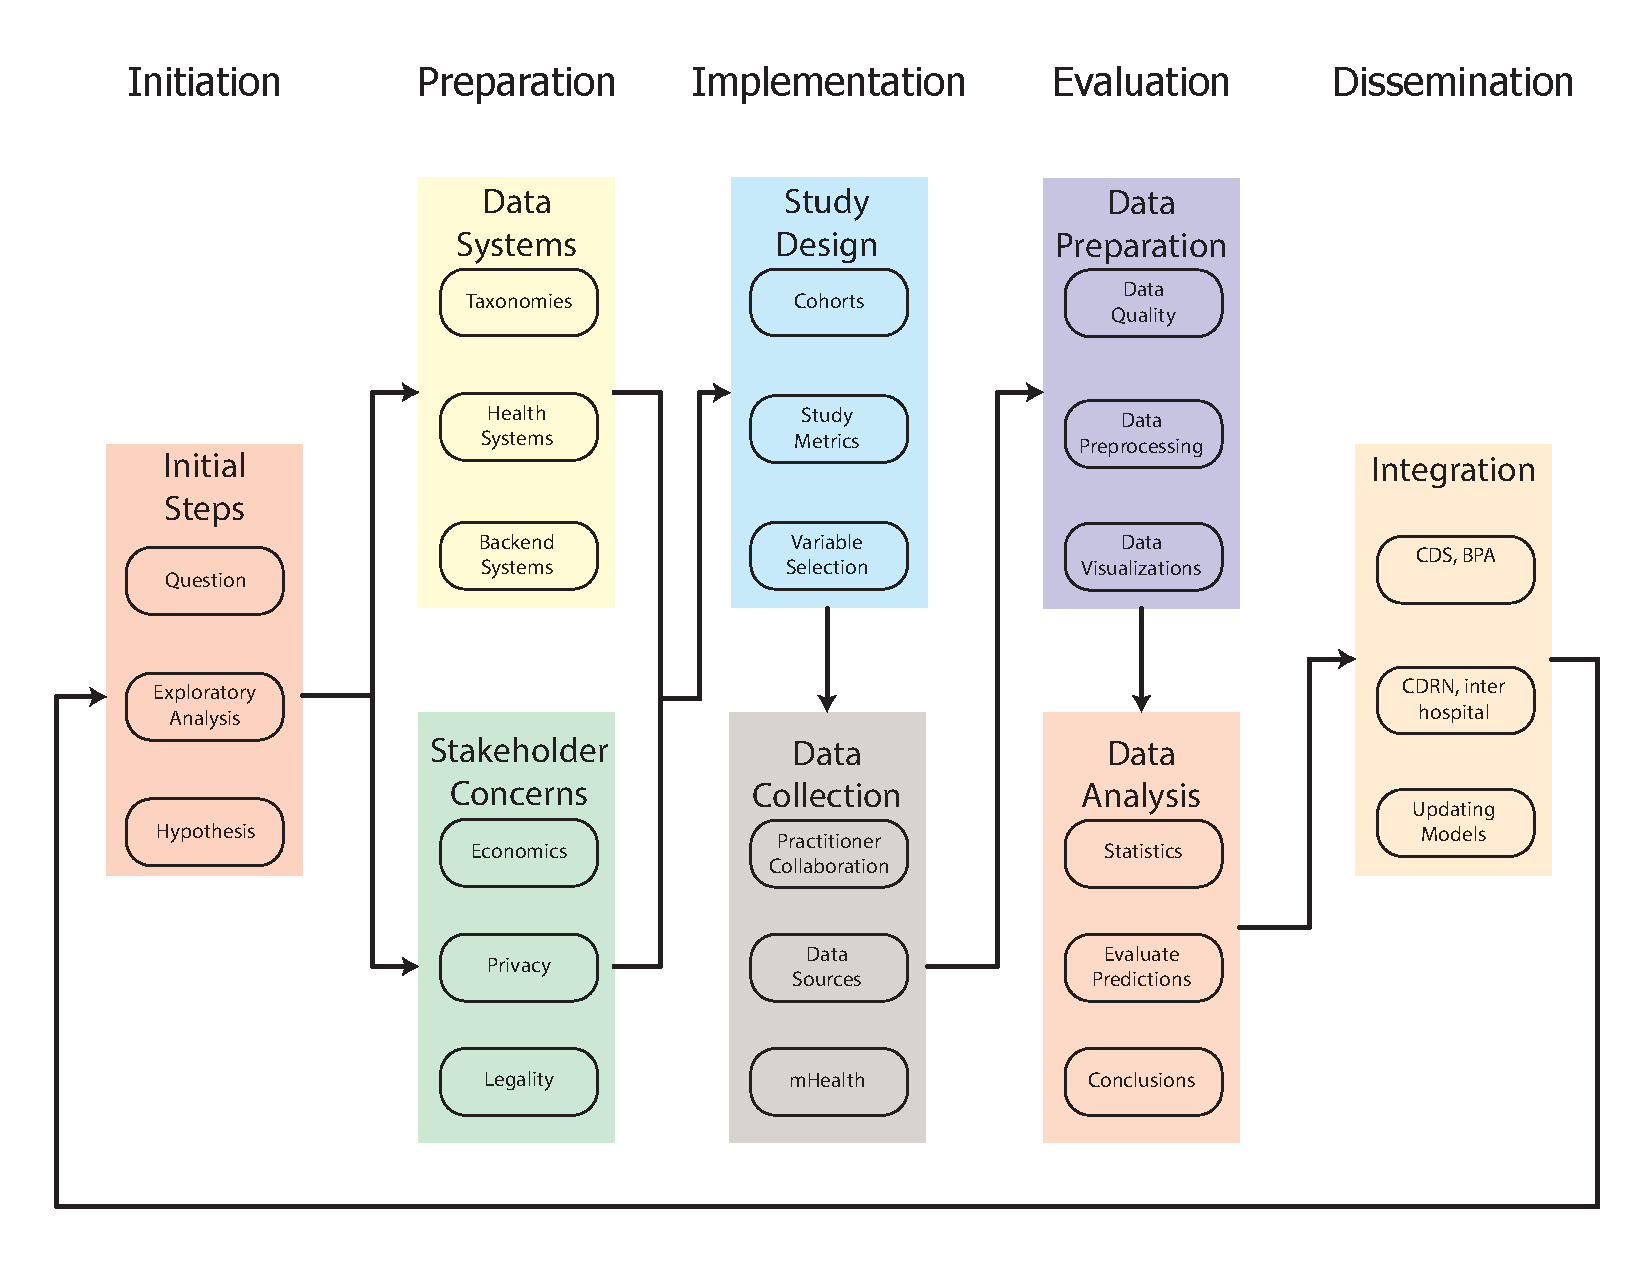
\includegraphics[height=\textheight]{../../informatics_pipeline.pdf}
\end{frame}

\section{Metrics for Evaluation of Classification Models}

\begin{frame}{Terms and Questions}
	\begin{columns}[T]
		\begin{column}{0.4\textwidth}\centering
			\textbf{Terms}
			\begin{itemize}
				\item Accuracy
				\item Specificity
				\item Sensitivity
				\item Positive Predictive Value 
				\item Negative Predictive Value 
				\item Likelihood Ratio
				\item ROC \& AUC
				\item F1 Score
			\end{itemize}
		\end{column}
		\begin{column}{0.6\textwidth}\centering
			\textbf{Questions}
			\onslide<2>{
			\begin{itemize}
				\item Is accuracy a useful metric?
				\item What information is conveyed by sensitivity vs specificity ?
				\item What information do the PPV and NPV add?
				\item Intuitively, how do sensitivity, specificity, likelihood ratios and ROC connect?
				\item Is the F1 score a more robust metric than the ROC and AUC?				
			\end{itemize}}
		\end{column}	
	\end{columns}
\end{frame}

\begin{frame}{Clinical Cases}
	\begin{itemize}
		\item Low dose CT for detecting lung cancer (LDCT)\footnote{National Lung Screening Trial Research Team. (2011). Reduced lung-cancer mortality with low-dose computed tomographic screening. New England Journal of Medicine, 365(5), 395-409.}
		\item Ultrasound detection of abdominal aortic aneurysms (AAA)\footnote{Thompson, S. G., Ashton, H. A., Gao, L., Buxton, M. J., Scott, R. A. P., \& Multicentre Aneurysm Screening Study (MASS) Group. (2012). Final follow‐up of the Multicentre Aneurysm Screening Study (MASS) randomized trial of abdominal aortic aneurysm screening. British Journal of Surgery, 99(12), 1649-1656.}
		\item Blood pressure monitoring in adolescents using home machines (HTN)\footnote{Stergiou, G. S., Nasothimiou, E., Giovas, P., Kapoyiannis, A., \& Vazeou, A. (2008). Diagnosis of hypertension in children and adolescents based on home versus ambulatory blood pressure monitoring. Journal of hypertension, 26(8), 1556-1562.}
		\item Detecting suicidality among adolescent outpatients by clinicians versus trained raters using the Kiddie Schedule for Affective Disorders and Schizophrenia (K-SADS-PL) \footnote{Holi, M. M., Pelkonen, M., Karlsson, L., Tuisku, V., Kiviruusu, O., Ruuttu, T., \& Marttunen, M. (2008). Detecting suicidality among adolescent outpatients: evaluation of trained clinicians' suicidality assessment against a structured diagnostic assessment made by trained raters. BMC psychiatry, 8(1), 97.}
	\end{itemize}
\end{frame}





\begin{frame}{Confusion Matrix}
	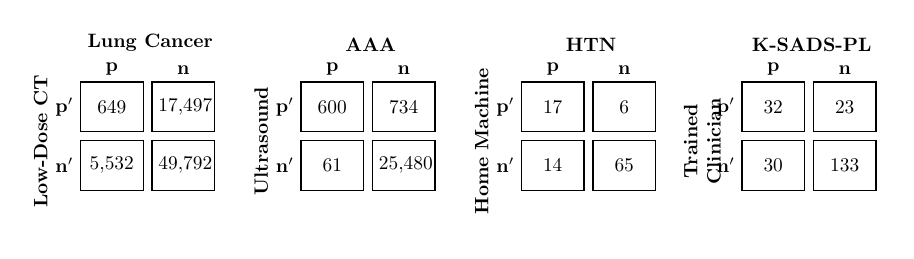
\begin{tikzpicture}[ampersand replacement=\&, scale=0.7, box/.style={draw, rectangle,minimum size=0.9cm,text width=0.9cm,align=center},  every node/.style={scale=0.7}]
		\begin{scope}
			\matrix (conmat) [row sep=.1cm,column sep=.1cm] {
				\node (tpos) [box, label=left:\( \mathbf{p'} \),label=above:\( \mathbf{p} \)] {649}; 	\&
				\node (fpos) [box, label=above:\textbf{n}] {17,497};	\\
				\node (fneg) [box, label=left:\( \mathbf{n'} \)] {5,532};	\&
				\node (tneg) [box] {49,792};	\\
				};
			\node [rotate=90, anchor=center,xshift=1cm, left=0.5cm of tpos, text width=3cm,align=center ] {\textbf{Low-Dose CT}};
			\node [above=0.3cm of fpos,xshift=-0.6cm,align=left] {\textbf{Lung Cancer}};
		\end{scope}
		\begin{scope}[xshift=4cm]
			\matrix (conmat) [row sep=.1cm,column sep=.1cm] {
				\node (tpos) [box, label=left:\( \mathbf{p'} \),label=above:\( \mathbf{p} \)] {600}; 	\&
				\node (fpos) [box, label=above:\textbf{n}] {734};	\\
				\node (fneg) [box, label=left:\( \mathbf{n'} \)] {61};	\&
				\node (tneg) [box] {25,480};	\\
				};
			\node [rotate=90, anchor=center,xshift=1cm, left=0.5cm of tpos, text width=3cm,align=center ] {\textbf{Ultrasound}};
			\node [above=0.3cm of fpos,xshift=-0.6cm,align=left] {\textbf{AAA}};
		\end{scope}
		\begin{scope}[xshift=8cm]
			\matrix (conmat) [row sep=.1cm,column sep=.1cm] {
				\node (tpos) [box, label=left:\( \mathbf{p'} \),label=above:\( \mathbf{p} \)] {17}; 	\&
				\node (fpos) [box, label=above:\textbf{n}] {6};	\\
				\node (fneg) [box, label=left:\( \mathbf{n'} \)] {14};	\&
				\node (tneg) [box] {65};	\\
				};
			\node [rotate=90, anchor=center,xshift=1cm, left=0.5cm of tpos, text width=3cm,align=center ] {\textbf{Home Machine}};
			\node [above=0.3cm of fpos,xshift=-0.6cm,align=left] {\textbf{HTN}};
		\end{scope}
		\begin{scope}[xshift=12cm]
			\matrix (conmat) [row sep=.1cm,column sep=.1cm] {
				\node (tpos) [box, label=left:\( \mathbf{p'} \),label=above:\( \mathbf{p} \)] {32}; 	\&
				\node (fpos) [box, label=above:\textbf{n}] {23};	\\
				\node (fneg) [box, label=left:\( \mathbf{n'} \)] {30};	\&
				\node (tneg) [box] {133};	\\
				};
			\node [rotate=90, anchor=center,xshift=1cm, left=0.5cm of tpos, text width=3cm,align=center ] {\textbf{Trained Clinician}};
			\node [above=0.3cm of fpos,xshift=-0.6cm,align=left] {\textbf{K-SADS-PL}};
		\end{scope}		
	\end{tikzpicture}
		\begin{itemize}
			\item<2-> What is the accuracy of these tests?
			\item<3-> Are these good screening tests and/or diagnostic tests?
			\item<4-> How does the PPV and NPV affect your opinion of their utility?
			\item<5-> When are sensitivity, specificity, PPV and NPV appropriate tests?
			\item<6-> How are sensitivity, specificity, PPV and NPV affected by prevalence?
		\end{itemize}
\end{frame}

\note{\begin{table}
	\scriptsize
	\begin{tabular}{c c c}
		Parameter & Interpretation & Appropriate for \\ \hline \hline
		Accuracy &  Overall proximity of test to reality & Balanced sample sizes \\
		Sensitivity  & Chance of a false negative &  Cheap testing/Severe disease\\ 
		Specificity  &  Chance of a false positive &  Expensive testing/Mild disease\\
		PPV  & Sensitivity diagnostic utility & Balanced prevalence \\
		NPV & Specificity diagnostic utility & Balanced prevalence \\
	\end{tabular}
\end{table}

	\begin{table}
	\scalebox{0.9}{
		\begin{tabular}{| c | c | c | c | c | c | c | c | c | c | c |}
			\hline
			\textbf{Case} & \textbf{TP} & \textbf{FP} & \textbf{TN} & \textbf{FN} & \textbf{Sens} & \textbf{Spec} & \textbf{PPV} & \textbf{NPV} & \textbf{Acc} & \textbf{F1} \\ \hline
			LDCT& 649 & 17,497 & 49,792 & 5,532 & 10 & 74 & 4 & 90  & 69 & 6\\ \hline
			AAA & 600 & 734 & 25,480 & 61 & 91 & 97 & 45 & 100  & 97 & 60\\ \hline
			HTN & 17 & 6 & 65 & 14 & 55 & 92 & 74 & 82  & 80 & 63\\ \hline
			KSADS & 32 & 23 & 133 & 30 & 52 & 85 & 58 & 82 & 76 & 55\\ \hline
		\end{tabular}
		}
	\end{table}
	
	}



\begin{frame}{Combined Statistics}
	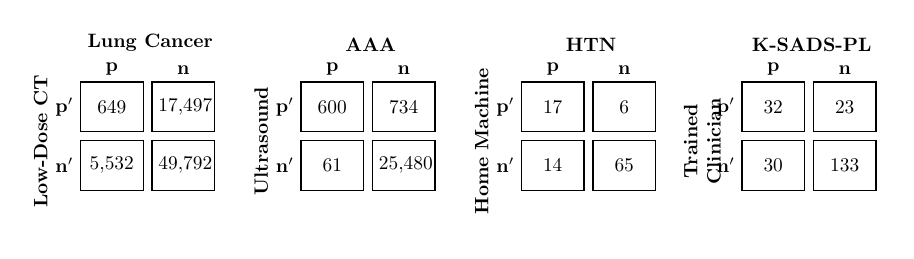
\begin{tikzpicture}[ampersand replacement=\&, scale=0.7, box/.style={draw, rectangle,minimum size=0.9cm,text width=0.9cm,align=center},  every node/.style={scale=0.7}]
		\begin{scope}
			\matrix (conmat) [row sep=.1cm,column sep=.1cm] {
				\node (tpos) [box, label=left:\( \mathbf{p'} \),label=above:\( \mathbf{p} \)] {649}; 	\&
				\node (fpos) [box, label=above:\textbf{n}] {17,497};	\\
				\node (fneg) [box, label=left:\( \mathbf{n'} \)] {5,532};	\&
				\node (tneg) [box] {49,792};	\\
				};
			\node [rotate=90, anchor=center,xshift=1cm, left=0.5cm of tpos, text width=3cm,align=center ] {\textbf{Low-Dose CT}};
			\node [above=0.3cm of fpos,xshift=-0.6cm,align=left] {\textbf{Lung Cancer}};
		\end{scope}
		\begin{scope}[xshift=4cm]
			\matrix (conmat) [row sep=.1cm,column sep=.1cm] {
				\node (tpos) [box, label=left:\( \mathbf{p'} \),label=above:\( \mathbf{p} \)] {600}; 	\&
				\node (fpos) [box, label=above:\textbf{n}] {734};	\\
				\node (fneg) [box, label=left:\( \mathbf{n'} \)] {61};	\&
				\node (tneg) [box] {25,480};	\\
				};
			\node [rotate=90, anchor=center,xshift=1cm, left=0.5cm of tpos, text width=3cm,align=center ] {\textbf{Ultrasound}};
			\node [above=0.3cm of fpos,xshift=-0.6cm,align=left] {\textbf{AAA}};
		\end{scope}
		\begin{scope}[xshift=8cm]
			\matrix (conmat) [row sep=.1cm,column sep=.1cm] {
				\node (tpos) [box, label=left:\( \mathbf{p'} \),label=above:\( \mathbf{p} \)] {17}; 	\&
				\node (fpos) [box, label=above:\textbf{n}] {6};	\\
				\node (fneg) [box, label=left:\( \mathbf{n'} \)] {14};	\&
				\node (tneg) [box] {65};	\\
				};
			\node [rotate=90, anchor=center,xshift=1cm, left=0.5cm of tpos, text width=3cm,align=center ] {\textbf{Home Machine}};
			\node [above=0.3cm of fpos,xshift=-0.6cm,align=left] {\textbf{HTN}};
		\end{scope}
		\begin{scope}[xshift=12cm]
			\matrix (conmat) [row sep=.1cm,column sep=.1cm] {
				\node (tpos) [box, label=left:\( \mathbf{p'} \),label=above:\( \mathbf{p} \)] {32}; 	\&
				\node (fpos) [box, label=above:\textbf{n}] {23};	\\
				\node (fneg) [box, label=left:\( \mathbf{n'} \)] {30};	\&
				\node (tneg) [box] {133};	\\
				};
			\node [rotate=90, anchor=center,xshift=1cm, left=0.5cm of tpos, text width=3cm,align=center ] {\textbf{Trained Clinician}};
			\node [above=0.3cm of fpos,xshift=-0.6cm,align=left] {\textbf{K-SADS-PL}};
		\end{scope}		
	\end{tikzpicture}
	\begin{itemize}[<+(0)->]
		\item What are 4 'sensible' pairings of the base stats
		\item What are the different ways to combine the base stats into summary statistics (hint: what are the basic ways to combine any numbers)?
		\begin{itemize}
			\item<.-> Work through each of the four clinical cases
		\end{itemize}
		\item What determines the split of positive cases into TP vs FN and negative cases into TN vs FP? 
	\end{itemize}
\end{frame}

\note{
	\scriptsize
	\begin{itemize}
		\item sens/spec, PPV/NPV, sens/PPV, spec/NPV
		\item the 4 basic operations are add, subtract, multiply and divide \textbf{add Ex}
		\item \textbf{Add} adding just gives you the numbers themselves without an idea of how they each contribute. averaging sens/spec or ppv/npv is a good summary of how they perform.  Averaging sens/ppv tells you how well you can predict TP taking into account the reliability of the test and the prevalence of the disease, and specifically ignoring the effects of TN.  
		\item \textbf{Subtract} Not really a helpful metric as the difference between values doesn't tell you much about the values themselves.  F1 score combines the typical mean and the difference between the values
		\item \textbf{multiply} Similar to averaging and F1 but punishes if both lower values
		\item \textbf{divide} dividing two probabilities gives you an odds ratio, i.e., how much more likely the numerator is to happen than the denominator.  
		
	\end{itemize}
}
%$LR+ &= \dfrac{sensitivity}{1 - specificity} = \dfrac{P\left(T+ \mid D+\right)}{P\left(T+ \mid D-\right)}$
%$LR- &= \dfrac{1 - sensitivity}{specificity} = \dfrac{P\left(T- \mid D+\right)}{P\left(T- \mid D-\right)}$
\note{
	\scriptsize
	\begin{columns}[T]
		\begin{column}{0.5\textwidth}\centering		
			$LR+ = \dfrac{sensitivity}{1 - specificity} = \dfrac{P\left(T+ \mid D+\right)}{P\left(T+ \mid D-\right)}$
		\end{column}
		\begin{column}{0.5\textwidth}\centering		
			$LR- = \dfrac{1 - sensitivity}{specificity} = \dfrac{P\left(T- \mid D+\right)}{P\left(T- \mid D-\right)}$
		\end{column}
	\end{columns}
		
	\begin{center}
		\rowcolors{2}{gray!25}{white}
		\begin{tabular}{c c}
			\rowcolor{gray!50}
			Likelihood Ratio & Approximate Change in Probability(\%) \\ \hline
			0.1 & -45 \\
			0.2 & -30 \\
			0.5 & -15 \\
			1 & 0 \\
			2 & +15 \\
			5 & +30 \\
			10 & +45
		\end{tabular} \\[2em]
		Change in post test probability $\approx 0.2 \times \ln{LR}$ \\
		\tiny{McGee, Steven. "Simplifying likelihood ratios." Journal of general internal medicine 17.8 (2002): 647-650.
APA	
}
	\end{center}
}









\begin{frame}{Hypothesis Testing}
	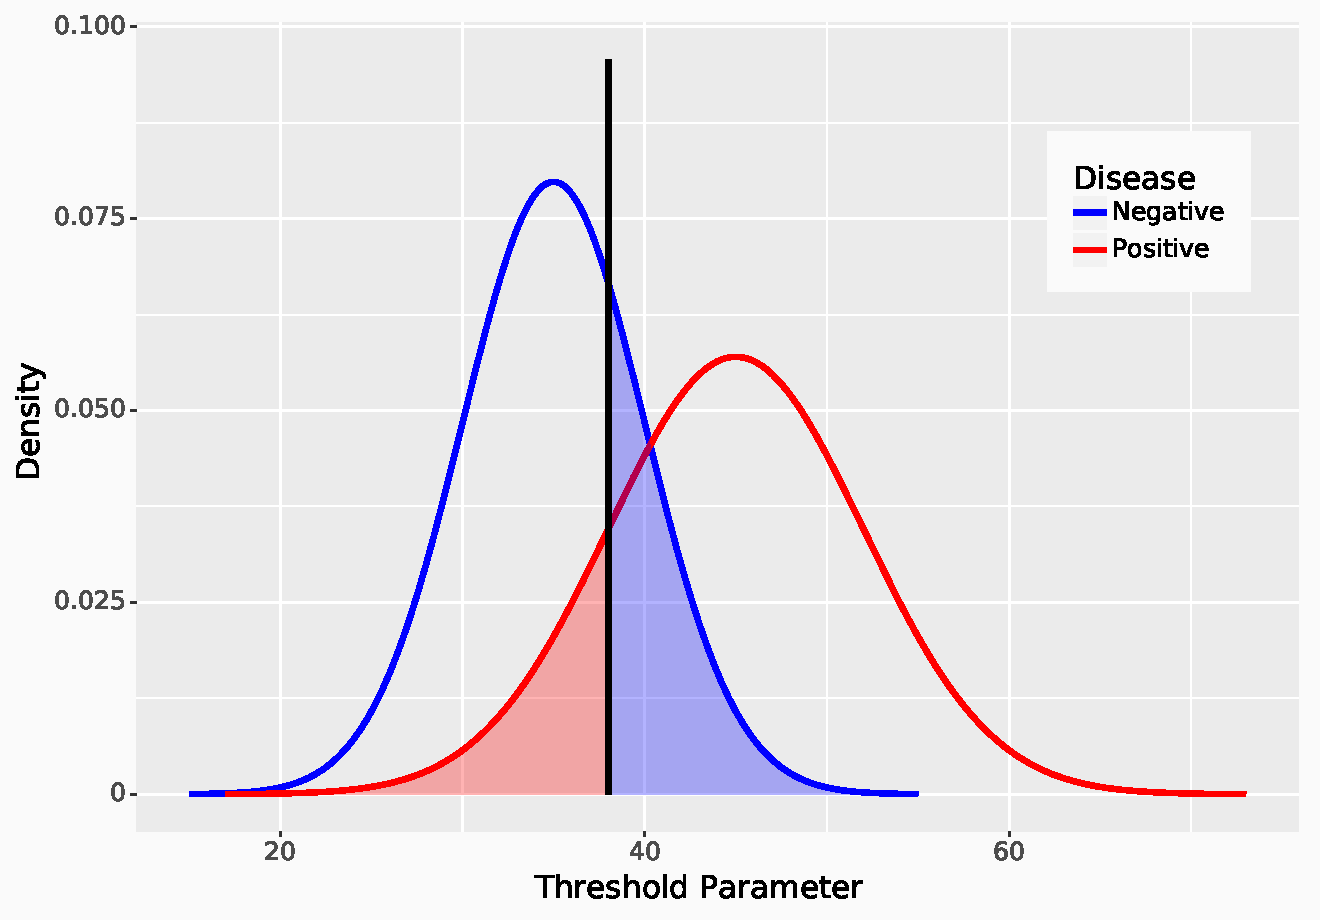
\includegraphics[height=0.85\textheight]{images/overlap_distr.pdf}
\end{frame}

\note{
	\begin{itemize}
		\item these two curves represent the positive and negative cases
		\item As the threshold parameter from right to left, your sensitivity increases but you specificity decreases
		\item In order to calculate specific values we need to know what the areas under the curve are, for different thresholds
	\end{itemize}
}

\begin{frame}{Hypothesis Testing}
	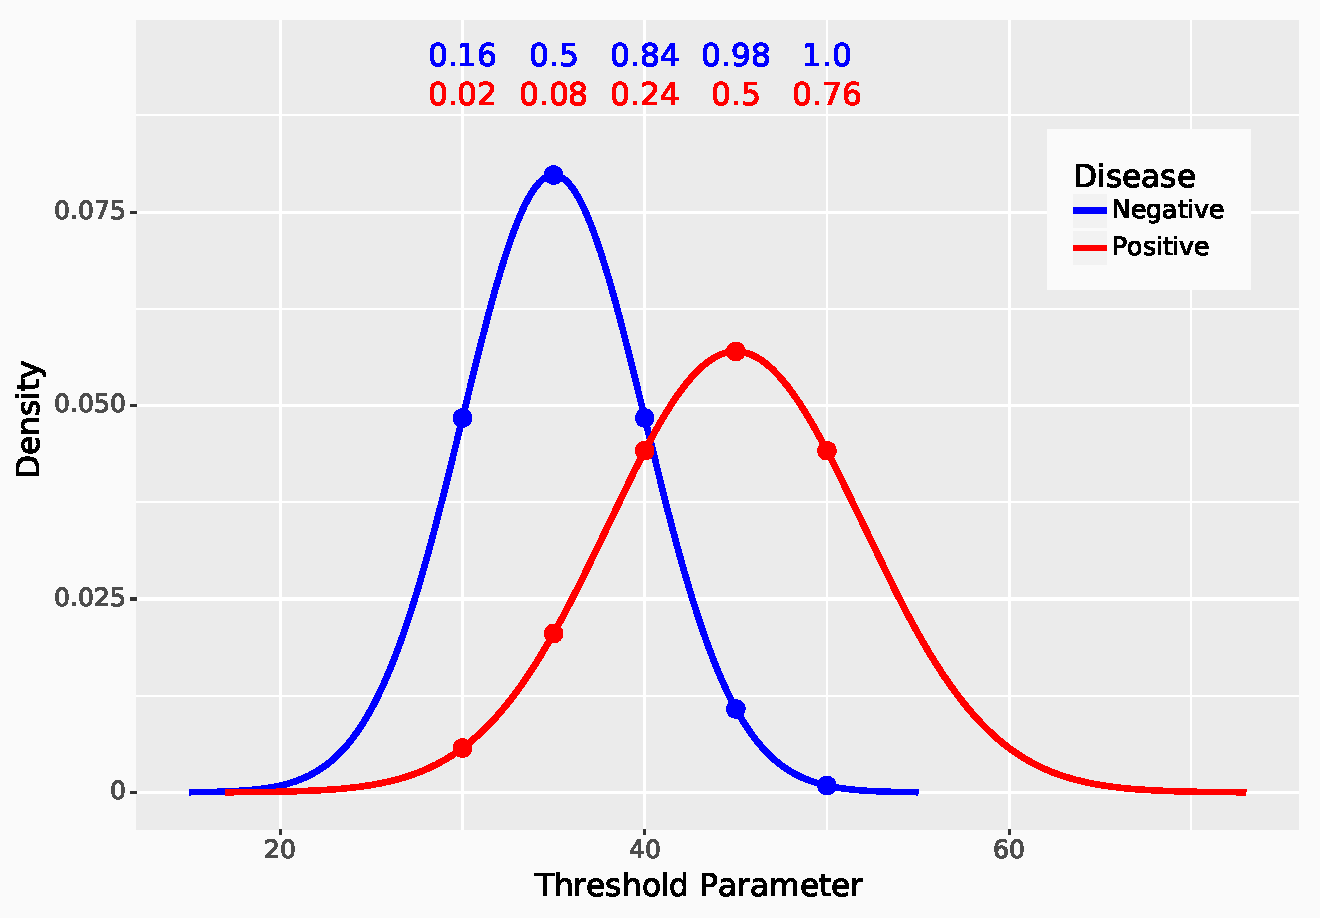
\includegraphics[height=0.85\textheight]{images/overlap_distr_points.pdf}
\end{frame}

\note{
	\begin{itemize}
		\item Let's calculate the odds ratio for various points along the curve 
	\end{itemize}
	\vspace{-2em}
	\begin{table}
		\scalebox{0.6}{
		\begin{tabular}{| c | c | c | c | c | c | c |}
			\hline
			\textbf{N/P} & \textbf{Sens} & \textbf{Spec} & \textbf{Odds} & \textbf{PPV} & \textbf{NPV} & \textbf{F1} \\ \hline
			0.16/002 & 0.98 & 0.16 & 1.17 & 0.54 & 0.89 & 0.70\\ \hline
			0.5/0.08 & 0.92 & 0.50 & 1.84 & 0.65 & 0.86 & 0.76\\ \hline
			0.84/0.24 & 0.76 & 0.84 & 4.78 & 0.83 & 0.78 & 0.79\\ \hline
			0.98/0.5 & 0.50 & 0.98 & 26.32 & 0.96 & 0.66 & 0.66\\ \hline
			1.0/0.76 & 0.24 & 1.00 & $\infty$ & 1 & 0.57 & 0.39\\ \hline
		\end{tabular}
		}
	\end{table}
	\vspace{-2em}
	\begin{table}
		\scalebox{0.6}{
		\begin{tabular}{| c | c | c | c | c | c | c |}
			\hline
			\textbf{N/P} & \textbf{PPV-25\%P} & \textbf{NPV-25\%P} & \textbf{PPV-75\%P} & \textbf{NPV-75\%P} & \textbf{f1-25\%P} & \textbf{f1-75\%P} \\ \hline
			0.16/002 & 0.28 & 0.96 & 0.78 & 0.73 & 0.44 & 0.87\\ \hline
			0.5/0.08 & 0.38 & 0.95 & 0.85 & 0.68 & 0.54 & 0.88\\ \hline
			0.84/0.24 & 0.61 & 0.91 & 0.93 & 0.54 & 0.68 & 0.84\\ \hline
			0.98/0.5 & 0.89 & 0.86 & 0.99 & 0.40 & 0.64 & 0.66\\ \hline
			1.0/0.76 & 1 & 0.80 & 1.00 & 1 & 0.31 & 0.39\\ \hline
		\end{tabular}
		}
	\end{table}
	\begin{itemize}
		\item both of these curves have an area of 1, so we need to multiply each metric by the percentage of patients to see how prevalence affects the outcome
	\end{itemize}
}



%\begin{frame}{Receiver Operating Characteristic}
%	\begin{center}
%		 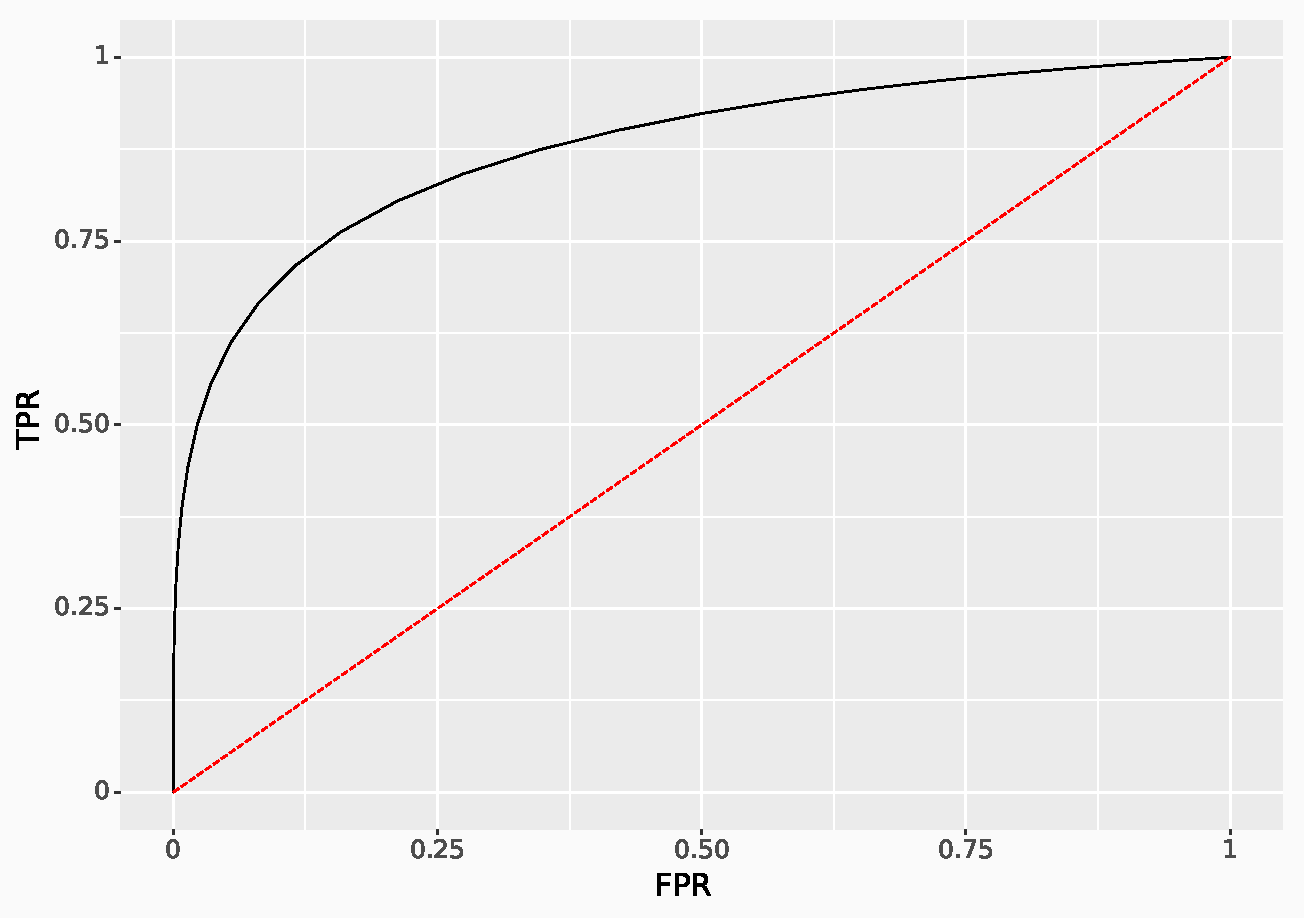
\includegraphics[height=0.8\textheight]{images/ROC.pdf}\\
%	\end{center}
%\end{frame}

\begin{frame}{Receiver Operating Characteristic}
	\begin{center}
		 \stackinset{r}{1em}{b}{3em}{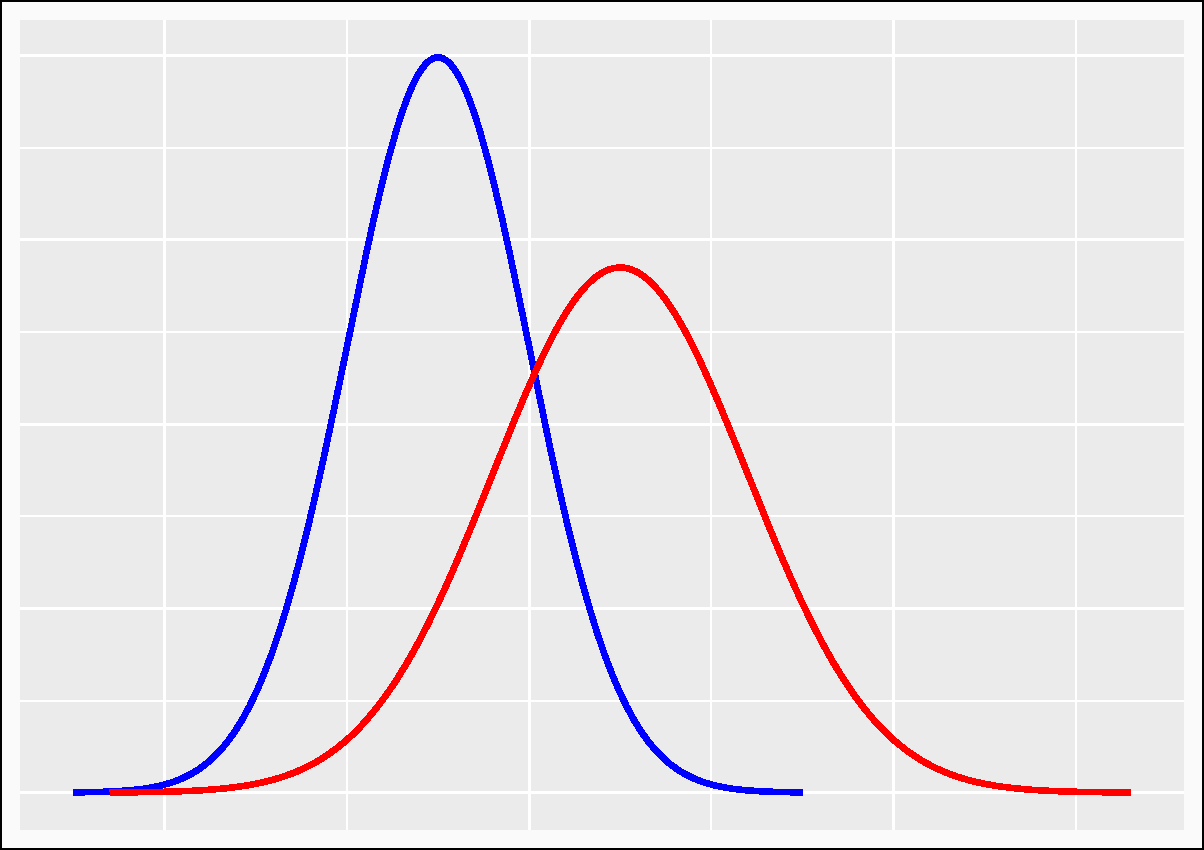
\includegraphics[width=1in]{images/overlap_distr_no_thresh.pdf}}
  {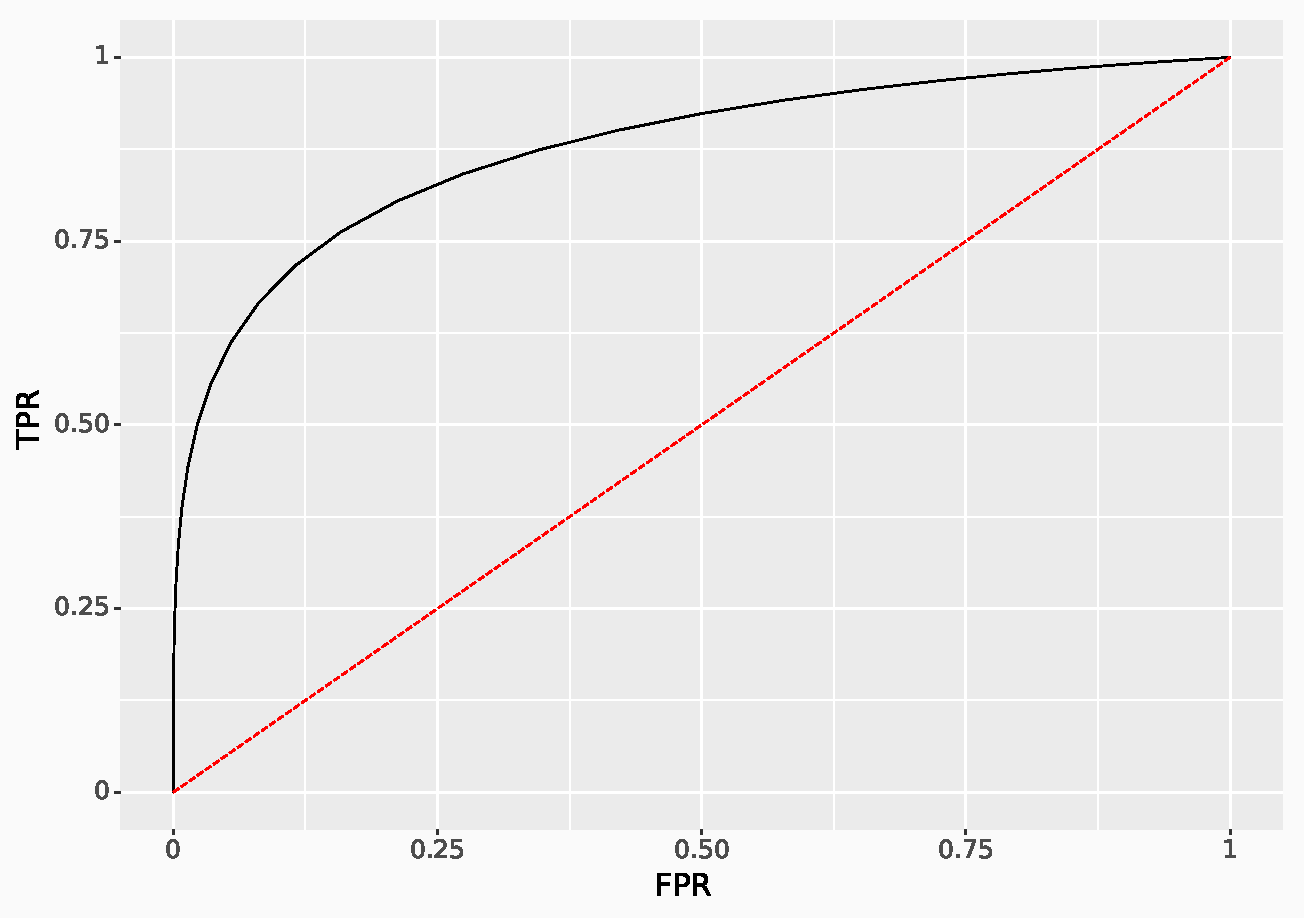
\includegraphics[width=1\textwidth]{images/ROC.pdf}}\\
	\end{center}
	\note[item]{What does the Area Under the Curve (AUC) correspond to? - Given a positive test result what are the chances that the subject is truly positive irrespective of prevalence?} 
  \note[item]{What does the diagonal correspond to? - equal probabilities}
	\note[item]{}	
	\note[item]{PPV is threshold dependent, while AUC is threshold independent but variable dependent}	
\end{frame}


\begin{frame}{Receiver Operating Characteristic}
	\begin{center}
		 \stackinset{r}{1em}{b}{3em}{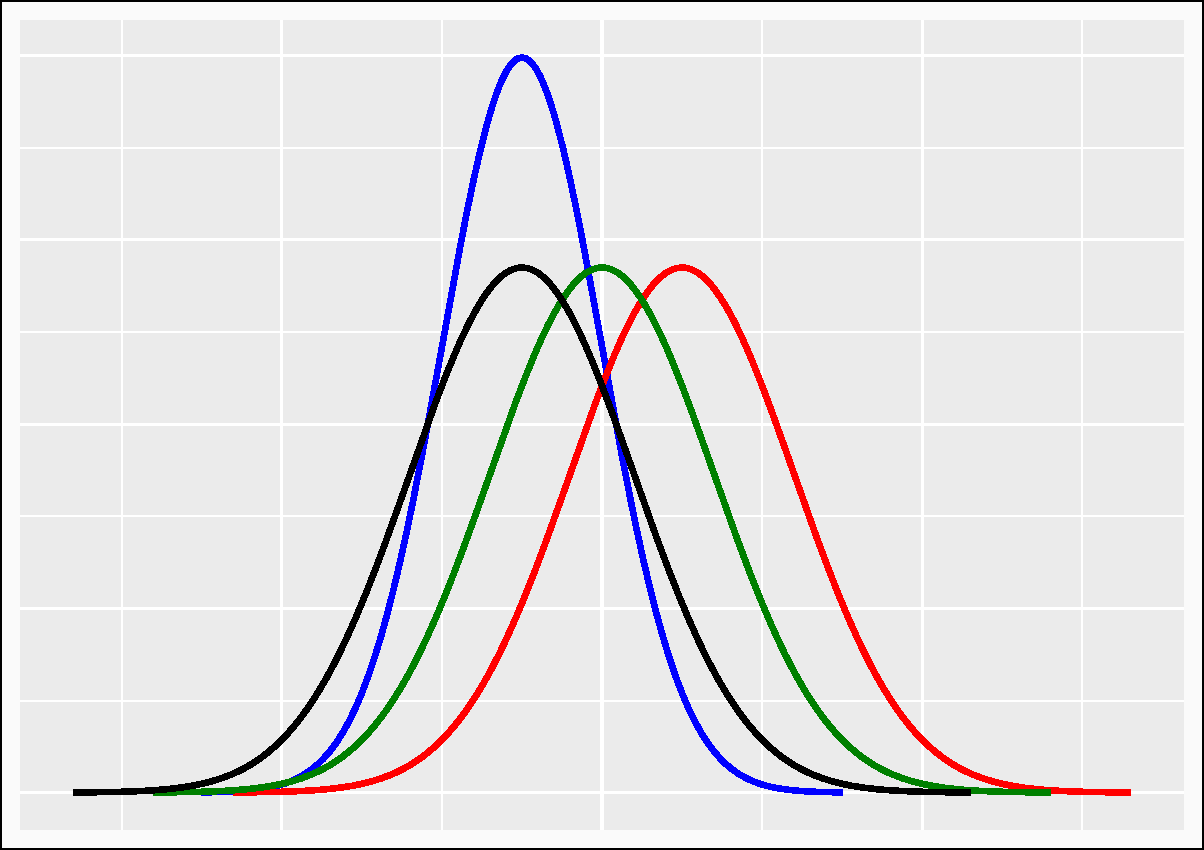
\includegraphics[width=1in]{images/overlap_distr_no_thresh_diff_sens.pdf}}
  {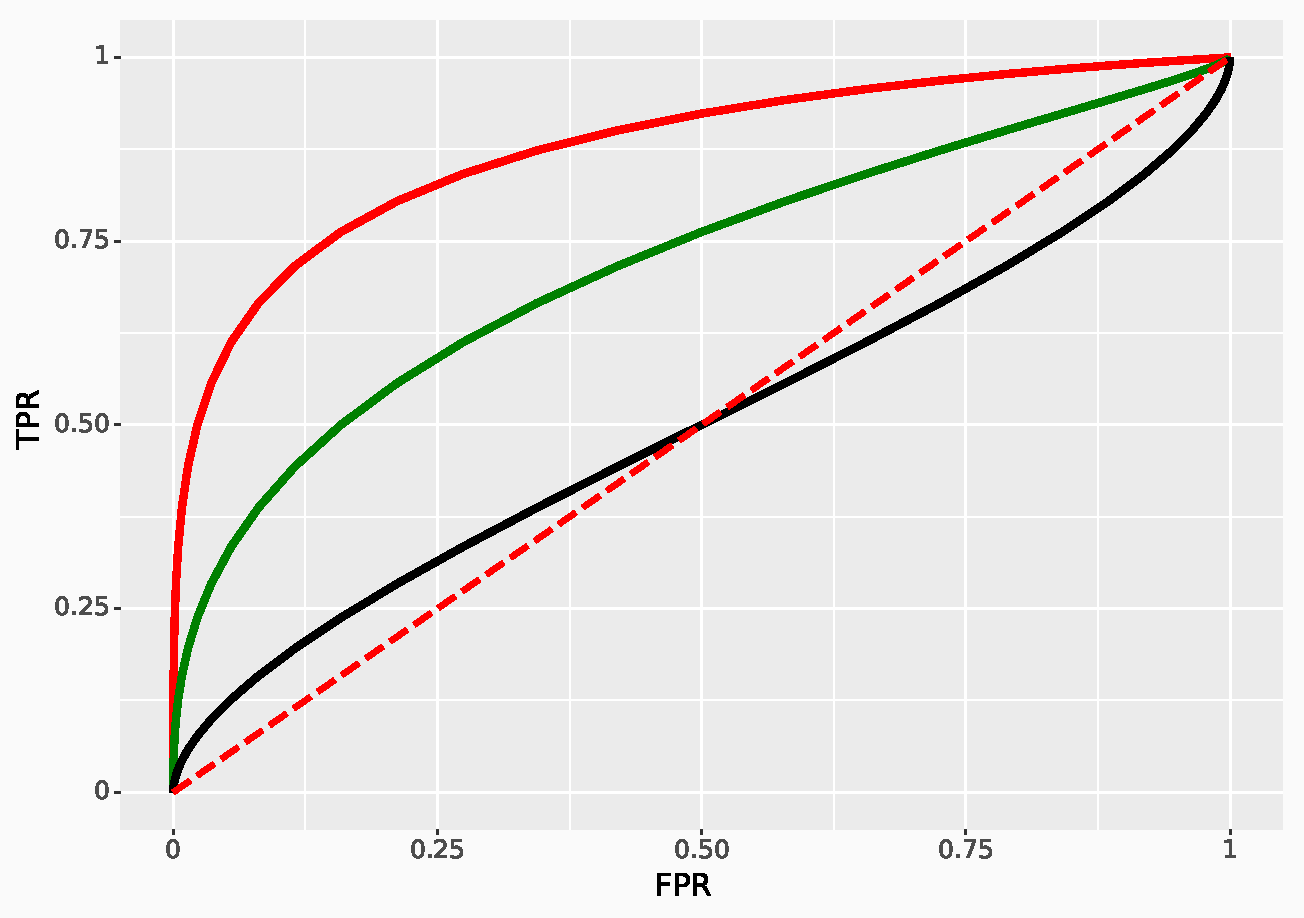
\includegraphics[width=1\textwidth]{images/ROC_dist_diff.pdf}}\\
	\end{center}
\end{frame}









\section{Metrics for Evaluation of Regression Models}

\begin{frame}{Regression Metrics}
	\begin{itemize}
		\item What aspects of a model's predictions should I care about?
		\item What aspects of the model's predictions can I evaluate? 
	\end{itemize}

	\note[item]{
		\begin{itemize}
			\item Accuracy (bias), precision (variance)
			\item Average distance of errors
			\item Worst case error
			\item Do large errors matter more than small errors
			\item Maximal distance of errors 
			\item Difference between my model and some standard model
		\end{itemize}
		}
	\note[item]{difference, squared difference, min/max, variance of predictions, relative difference (percentage error)}
\end{frame}





\begin{frame}{Regression Metrics}
	\begin{table}
		%\def\arraystretch{2}
		\begin{tabular}{| l | c | >{\tiny}Sl |}
		\hline
		\multirow{2}{2cm}{Equal weighting of errors} & MAE & $\dfrac{1}{n}\sum\limits_{i=0}^{n-1}\abs{y_i-\hat{y}_i}$ \\ \cline{2-3}
		& MAPE & $ \dfrac{100}{n}\sum\limits_{i=0}^{n-1}\dfrac{\abs{y_i-\hat{y}_i}}{y_i}$ \\ \hline
		\multirow{3}{2cm}{Unequal weighting of errors} & MSE & $\dfrac{1}{n}\sum\limits_{i=0}^{n-1}\left(y_i-\hat{y}_i\right)^2$ \\ \cline{2-3}
		& RMSE & $\sqrt{\dfrac{1}{n}\sum\limits_{i=0}^{n-1}\left(y_i-\hat{y}_i\right)^2}$ \\\cline{2-3}
		& MSLE & $\dfrac{1}{n}\sum\limits_{i=0}^{n-1}\left(\ln \left(1=y_i\right)-\ln\left(1+\hat{y}_i\right)\right)^2$ \\ \hline
		\multirow{2}{2cm}{Data Variance} & $R^2$ & $1 - \frac{\sum\limits_{i=0}^{n-1}\left(y_i-\hat{y}_i\right)^2}{\sum\limits_{i=0}^{n-1}\left(y_i-\bar{y}_i\right)^2}$ \\ \cline{2-3}
		& Explained Var & $1-\dfrac{Var\left(y-\hat{y}\right)}{Var\left(y\right)}$\\ \hline
		\end{tabular}
	\end{table}

\end{frame}

\section{Data Quality}

\begin{frame}{Factors Which Affect Data Quality}
	\begin{center}
		Analysis is only ever as good as the data its built upon.
	\end{center}
	\begin{itemize}
		\item<2-> Data Definition
		\item<2-> Data Collection
		\item<2-> Data Processing
		\item<2-> Data Representation
	\end{itemize}
\end{frame}


\begin{frame}{How Can Data Be Wrong}
	\begin{itemize}
		\item Incomplete
		\item Inconsistent
		\item Inaccurate
	\end{itemize}
\end{frame}

\begin{frame}{Processes to Assure Data Quality}
	\begin{itemize}
		\item Data Provenance
		\item Sanity Checks
		\item Exploratory Data Analysis		
	\end{itemize}
\end{frame}


\section{Old Slides}

\begin{frame}{Clinical Cases}
	\begin{table}
		\begin{tabular}{| c | c | c | c | c | c | c | c | c |}
			\hline
			\textbf{Case} & \textbf{TP} & \textbf{FP} & \textbf{TN} & \textbf{FN} \\ \hline
			LDCT & 649 & 17,497 & 49,792 & 5,532  \\ \hline
			AAA & 600 & 734 & 25,480 & 61  \\ \hline
			HTN & 17 & 6 & 65 & 14 \\ \hline
		\end{tabular}
	\end{table}
	\begin{itemize}
		\item<2-> Are these \textit{good} tests?
		\item<2-> In what contexts are they useful?
		\item<2-> For which metrics are they misleading?
	\end{itemize}
\end{frame}

\begin{frame}{Clinical Cases}
	\begin{table}
		\begin{tabular}{| c | c | c | c | c | c | c | c | c |}
			\hline
			\textbf{Case} & \textbf{TP} & \textbf{FP} & \textbf{TN} & \textbf{FN} & \textbf{Sens} & \textbf{Spec} & \textbf{PPV} & \textbf{NPV}  \\ \hline
			LDCT& 649 & 17,497 & 49,792 & 5,532 & 10 & 74 & 4 & 90  \\ \hline
			AAA & 600 & 734 & 25,480 & 61 & 91 & 97 & 45 & 100 \\ \hline
			HTN & 17 & 6 & 65 & 14 & 55 & 92 & 74 & 82 \\ \hline
		\end{tabular}
	\end{table}
\end{frame}

\begin{frame}{Confusion Matrix}
	\begin{center}
		\begin{tikzpicture}[transform canvas={scale=0.65}, ampersand replacement=\&, box/.style={draw, rectangle, minimum size=1cm, text width=2.75cm, align=center}, box2/.style={draw, rectangle, minimum size=1cm, text width=3.25cm, align=center}]
			\matrix (conmat) [row sep=.1cm,column sep=.1cm] {
				\node (tpos) [box, label=left:\( \mathbf{p'} \), label=above:\( \mathbf{p} \)] {TP}; \&
				\node (fpos) [box, label=above:\textbf{n}] {FP};\&
				\node (ppv) [box2] {PPV = {$p\left(\texttt{\textbf{p}}\mid \texttt{\textbf{p}}'\right)$}};\\
				\node (fneg) [box, label=left:\( \mathbf{n'} \)] {FN};\&
				\node (tneg) [box] {TN};\&
				\node (npv) [box2] {NPV = {$p\left(\texttt{\textbf{n}}\mid \texttt{\textbf{n}}'\right)$}};\\
				\node (sens) [box] {Sens = {$p\left(\texttt{\textbf{p}}'\mid \texttt{\textbf{p}}\right)$}};\&
				\node (spec) [box] {Spec = {$p\left(\texttt{\textbf{n}}'\mid \texttt{\textbf{n}}\right)$}};\&
				\node (acc) [box2] {Acc = {$p\left(TP + TN\right)$}};\\
			};
			\node [rotate=90, anchor=center,xshift=.35cm, left=1cm of tpos, text width=1.5cm,align=center ] {\textbf{predicted \\ outcome}};
			\node [above=0.5cm of fpos,xshift=-1.5cm,align=left] {\textbf{actual outcome}};
		\end{tikzpicture}
	\end{center}
	\vspace{3em}
	\only<2>{
		\begin{table}
			\scalebox{0.8}{
				\begin{tabular}{| c | c | c | c | c | c | c | c | c | c |}
					\hline
					\textbf{Case} & \textbf{TP} & \textbf{FP} & \textbf{TN} & \textbf{FN} & \textbf{Sens} & \textbf{Spec} & \textbf{PPV} & \textbf{NPV} & \textbf{Acc}   \\ \hline
					LDCT& 649 & 17,497 & 49,792 & 5,532 & &&& &  \\ \hline
					AAA & 600 & 734 & 25,480 & 61 & &&&& \\ \hline
					HTN & 17 & 6 & 65 & 14 & &&&& \\ \hline
				\end{tabular}
			}
		\end{table}
		\begin{center}
			Estimate if you think the value will be low, medium or high
		\end{center}	
	}
	\only<3>{
		\begin{table}
			\scalebox{0.9}{
				\begin{tabular}{| c | c | c | c | c | c | c | c | c | c |}
					\hline
					\textbf{Case} & \textbf{TP} & \textbf{FP} & \textbf{TN} & \textbf{FN} & \textbf{Sens} & \textbf{Spec} & \textbf{PPV} & \textbf{NPV} & \textbf{Acc} \\ \hline
					LDCT& 649 & 17,497 & 49,792 & 5,532 & 10 & 74 & 4 & 90  & 69 \\ \hline
					AAA & 600 & 734 & 25,480 & 61 & 91 & 97 & 45 & 100  & 97\\ \hline
					HTN & 17 & 6 & 65 & 14 & 55 & 92 & 74 & 82  & 80\\ \hline
				\end{tabular}
			}
		\end{table}
	}
\end{frame}







\begin{frame}{Confusion Matrix}
	\vspace{4em}
	\begin{center}
		\begin{tikzpicture}[transform canvas={scale=0.65}, ampersand replacement=\&, box/.style={draw, rectangle, minimum size=1cm, text width=2.75cm, align=center}, box2/.style={draw, rectangle, minimum size=1cm, text width=3.25cm, align=center}]
			\matrix (conmat) [row sep=.1cm,column sep=.1cm] {
				\node (tpos) [box, label=left:\( \mathbf{p'} \), label=above:\( \mathbf{p} \)] {TP}; \&
				\node (fpos) [box, label=above:\textbf{n}] {FP};\&
				\node (ppv) [box2] {PPV = {$p\left(\texttt{\textbf{p}}\mid \texttt{\textbf{p}}'\right)$}};\\
				\node (fneg) [box, label=left:\( \mathbf{n'} \)] {FN};\&
				\node (tneg) [box] {TN};\&
				\node (npv) [box2] {NPV = {$p\left(\texttt{\textbf{n}}\mid \texttt{\textbf{n}}'\right)$}};\\
				\node (sens) [box] {Sens = {$p\left(\texttt{\textbf{p}}'\mid \texttt{\textbf{p}}\right)$}};\&
				\node (spec) [box] {Spec = {$p\left(\texttt{\textbf{n}}'\mid \texttt{\textbf{n}}\right)$}};\&
				\node (acc) [box2] {Acc = {$p\left(TP + TN\right)$}};\\
			};
			\node [rotate=90, anchor=center,xshift=.35cm, left=1cm of tpos, text width=1.5cm,align=center ] {\textbf{predicted \\ outcome}};
			\node [above=0.5cm of fpos,xshift=-1.5cm,align=left] {\textbf{actual outcome}};
		\end{tikzpicture}
	\end{center}
	\vspace{3em}
	\begin{table}
		\scalebox{0.6}{
			\begin{tabular}{| c | c | c | c | c | c | c | c | c | c |}
				\hline
				\textbf{Case} & \textbf{TP} & \textbf{FP} & \textbf{TN} & \textbf{FN} & \textbf{Sens} & \textbf{Spec} & \textbf{PPV} & \textbf{NPV} & \textbf{Acc} \\ \hline
				LDCT& 649 & 17,497 & 49,792 & 5,532 & 10 & 74 & 4 & 90  & 69 \\ \hline
				AAA & 600 & 734 & 25,480 & 61 & 91 & 97 & 45 & 100  & 97\\ \hline
				HTN & 17 & 6 & 65 & 14 & 55 & 92 & 74 & 82  & 80\\ \hline
			\end{tabular}
		}
	\end{table}
	\begin{table}
		\scriptsize
		\begin{tabular}{c c c}
			Parameter & Interpretation & Appropriate for \\ \hline \hline
			Accuracy &  Overall proximity of test to reality & Balanced sample sizes \\
			Sensitivity  & \onslide<2>{Chance of a false negative} &  \onslide<2>{Cheap testing/Severe disease}\\ 
			Specificity  &  \onslide<2>{Chance of a false positive} &  \onslide<2>{Expensive testing/Mild disease}\\
			PPV  & \onslide<2>{Sensitivity diagnostic utility} & \onslide<2>{Balanced prevalence} \\
			NPV & \onslide<2>{Specificity diagnostic utility} & \onslide<2>{Balanced prevalence} \\
		\end{tabular}
	\end{table}
\end{frame}




\begin{frame}{Confusion Matrix}
	\vspace{4em}
	\begin{center}
		\begin{tikzpicture}[transform canvas={scale=0.75}, ampersand replacement=\&, box/.style={draw, rectangle, minimum size=1cm, text width=2.75cm, align=center}, box2/.style={draw, rectangle, minimum size=1cm, text width=3cm, align=center}]
			\matrix (conmat) [row sep=.1cm,column sep=.1cm] {
				\node (tpos) [box, label=left:\( \mathbf{p'} \), label=above:\( \mathbf{p} \)] {TP}; \&
				\node (fpos) [box, label=above:\textbf{n}] {FP};\&
				\node (ppv) [box2] {PPV = {$p\left(\texttt{\textbf{p}}\mid \texttt{\textbf{p}}'\right)$}};\\
				\node (fneg) [box, label=left:\( \mathbf{n'} \)] {FN};\&
				\node (tneg) [box] {TN};\&
				\node (npv) [box2] {NPV = {$p\left(\texttt{\textbf{n}}\mid \texttt{\textbf{n}}'\right)$}};\\
				\node (sens) [box] {Sens = {$p\left(\texttt{\textbf{p}}'\mid \texttt{\textbf{p}}\right)$}};\&
				\node (spec) [box] {Spec = {$p\left(\texttt{\textbf{n}}'\mid \texttt{\textbf{n}}\right)$}};\&
				\node (acc) [box2] {Acc = {$p\left(TP + TN\right)$}};\\
			};
			\node [rotate=90, anchor=center,xshift=.35cm, left=1cm of tpos, text width=1.5cm,align=center ] {\textbf{predicted \\ outcome}};
			\node [above=0.5cm of fpos,xshift=-1.5cm,align=left] {\textbf{actual outcome}};
		\end{tikzpicture}
	\end{center}
\vspace{3em}

	\begin{table}
		\scriptsize
		\begin{tabular}{c c c}
			Condition & Stats & Example \\ \hline \hline
			High Sensitivity, Low Specificity & \textbf{p}$'$ $>>$ \textbf{n}$'$ & test is always  positive \\	
			Low Sensitivity, High Specificity  & \textbf{n}$'$ $>>$ \textbf{p}$'$ & test is always negative \\
			High PPV, Low NPV & \textbf{p} $>>$ \textbf{n} & high disease prevalence \\
			Low PPV, High NPV & \textbf{n} $>>$ \textbf{p} & low disease prevalence \\
			High PPV, Low Sensitivity & FN $>>$ FP & say they are negative most of the time for a high prevalence disease \\
			High Sensitivity, Low NPV & & \\
			High Specificity, Low NPV & & \\
			High PPV, Low Specificity & & \\
		\end{tabular}
	\end{table}
\end{frame}

\begin{frame}{Combined Statistics}
	\begin{table}
		\scriptsize
		\begin{tabular}{c c c}
			Function of & Metric & Formula\\ \hline \hline \\ 
			Sensitivity, Specificity  & \textbf<2>{Positive Likelihood Ratio/ROC} & $\dfrac{sensitivity}{1-specificity}$ \\ [1.5em]
			Sensitivity, Specificity  & \textbf<2>{Negative Likelihood Ratio} & $\dfrac{1-sensitivity}{specificity}$ \\ [1.5em]
			Sensitivity, PPV & \textbf<2>{F1 score} & $\dfrac{2}{\dfrac{1}{sensitivity} + \dfrac{1}{PPV} }$  \\ [4em]
			TP, TN, FP, FN & Matthews correlation coefficient & \tiny{$\dfrac{TP\times TN-FP\times FN}{\sqrt{\left(TP + FP\right)\left(TP+FN\right)\left(TN+FP\right)\left(TN+FN\right)}}$} \\
		\end{tabular}
	\end{table}
\end{frame}


\begin{frame}{Likelihood Ratios}
	\begin{align*}
		LR+ &= \dfrac{sensitivity}{1 - specificity} = \dfrac{P\left(T+ \mid D+\right)}{P\left(T+ \mid D-\right)} \\[1.5em]
		LR- &= \dfrac{1 - sensitivity}{specificity} = \dfrac{P\left(T- \mid D+\right)}{P\left(T- \mid D-\right)}
	\end{align*}
	
\only<2>{
	\begin{center}
		Does a test result change the probability that a person has a certain condition?
	\end{center}}
\end{frame}


\begin{frame}{Likelihood Ratios}
	\begin{center}
		\rowcolors{2}{gray!25}{white}
		\begin{tabular}{c c}
			\rowcolor{gray!50}
			Likelihood Ratio & Approximate Change in Probability(\%) \\ \hline
			0.1 & -45 \\
			0.2 & -30 \\
			0.5 & -15 \\
			1 & 0 \\
			2 & +15 \\
			5 & +30 \\
			10 & +45
		\end{tabular} \\[2em]
		Change in post test probability $\approx 0.2 \times \ln{LR}$ \footnote{{McGee, Steven. "Simplifying likelihood ratios." Journal of general internal medicine 17.8 (2002): 647-650.
APA	
}}
	\end{center}
\end{frame}

\begin{frame}{Discrimination Thresholds}
	\begin{center}
		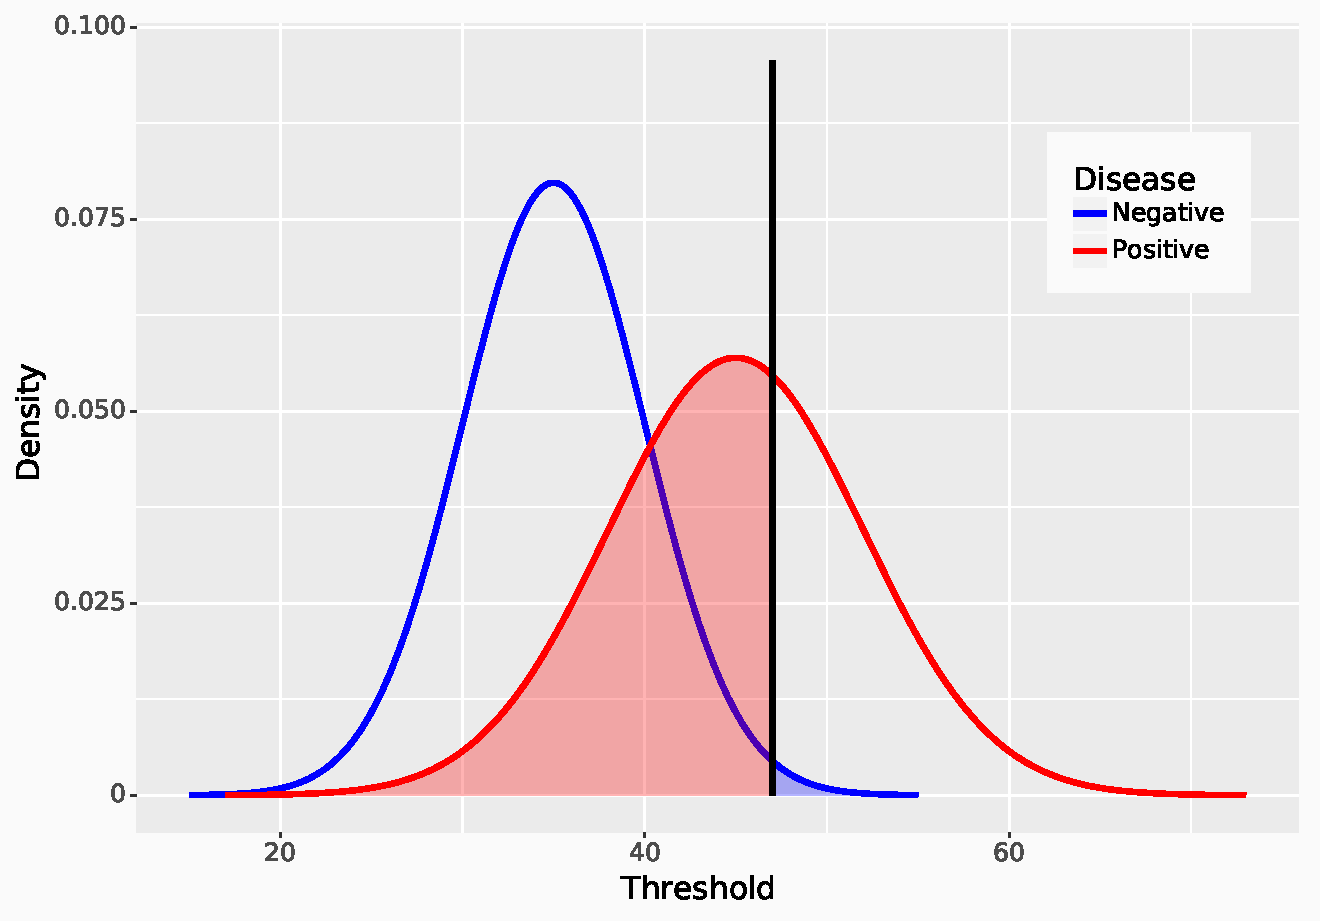
\includegraphics[height=0.45\textheight]{images/overlap_distr_thi.pdf}\\
		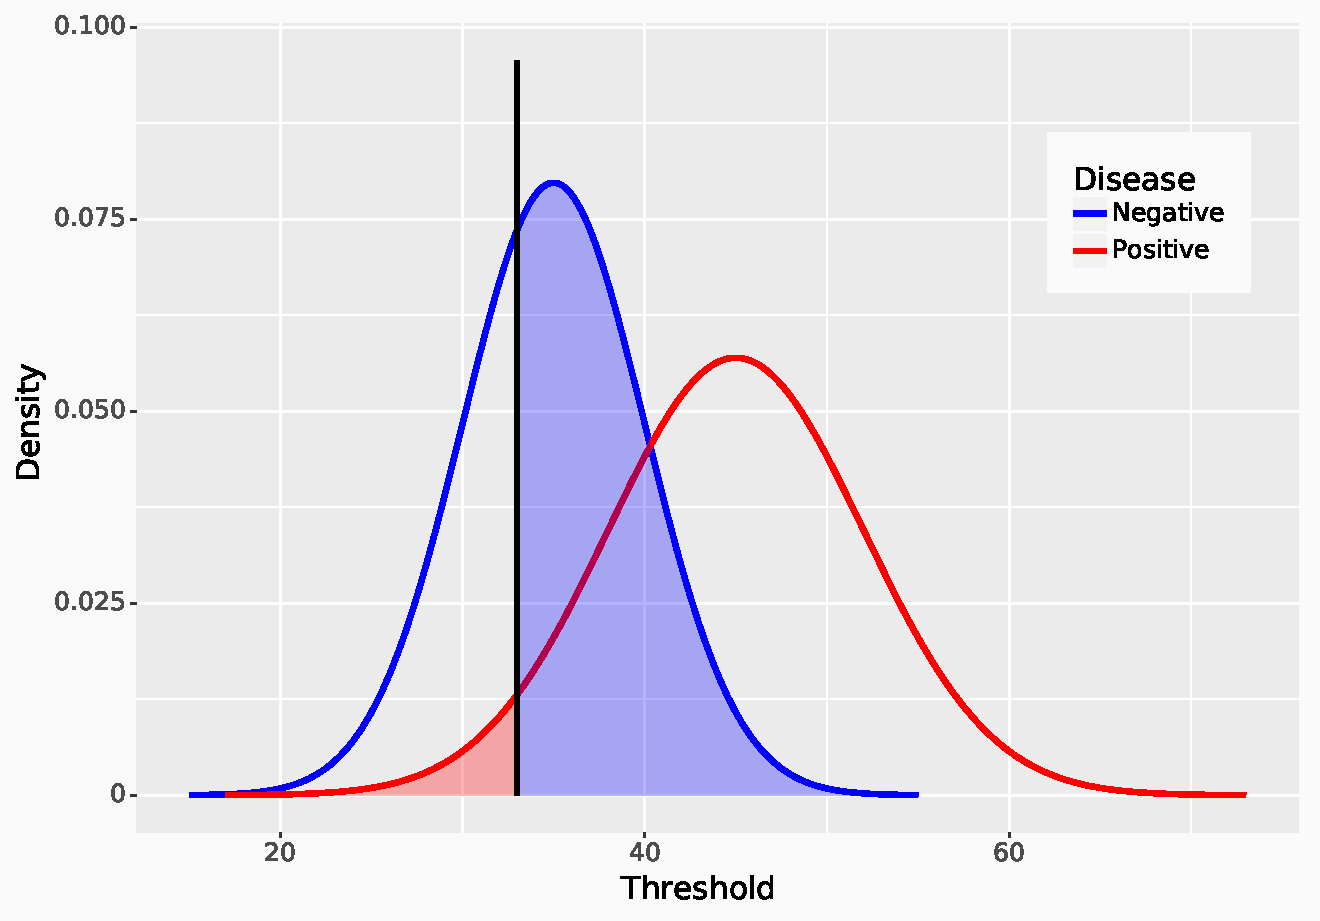
\includegraphics[height=0.45\textheight]{images/overlap_distr_tlow.pdf}
	\end{center}
\end{frame}

\begin{frame}{F1 Score}
\vspace{3em}
\begin{center}
\begin{tikzpicture}[transform canvas={scale=0.75}, ampersand replacement=\&,
box/.style={draw,rectangle,minimum size=1cm,text width=2.75cm,align=center},
box2/.style={draw,rectangle,minimum size=1cm,text width=3.25cm,align=center}]
\matrix (conmat) [row sep=.1cm,column sep=.1cm] {
\node (tpos) [box,
    label=left:\( \mathbf{p'} \),
    label=above:\( \mathbf{p} \),
    ] {TP};
\&
\node (fpos) [box,
    label=above:\textbf{n}] {FP};
\&
\node (ppv) [box2] {PPV = {$p\left(\texttt{\textbf{p}}\mid \texttt{\textbf{p}}'\right)$}};
\\
\node (fneg) [box,
    label=left:\( \mathbf{n'} \)] {FN};
\&
\node (tneg) [box] {TN};
\&
\node (npv) [box2] {NPV = {$p\left(\texttt{\textbf{n}}\mid \texttt{\textbf{n}}'\right)$}};
\\
\node (sens) [box] {Sens = {$p\left(\texttt{\textbf{p}}'\mid \texttt{\textbf{p}}\right)$}};
\&
\node (spec) [box] {Spec = {$p\left(\texttt{\textbf{n}}'\mid \texttt{\textbf{n}}\right)$}};
\&
\node (acc) [box2] {Acc = {$p\left(TP + TN\right)$}};
%\node (f1) [box2] {F1 = \scriptsize{$\dfrac{2 \times Sens \times PPV}{PPV + Sens}$}};
\\
};
\node [rotate=90, anchor=center,xshift=.35cm, left=1cm of tpos, text width=1.5cm,align=center ] {\textbf{predicted \\ outcome}};
\node [above=0.5cm of fpos,xshift=-1.5cm,align=left] {\textbf{actual outcome}};
\end{tikzpicture}
\end{center}
\vspace{1em}
	\begin{center}
		\begin{align*}
			F1 &= \dfrac{2}{\dfrac{1}{sensitivity} + \dfrac{1}{PPV} } = 2 \times \dfrac{PPV \cdot sensitivity}{PPV + sensitivity}
		\end{align*}\\[1em]
		How does F1 differ from AUC?
	\end{center}

\note[item]{F1 is sensitivity modified by prevalence.  So a low prevalence will hurt your F1 score but might not affect your AUC.  F1 is threshold specific and corresponds to a point on the ROC curve}	
	\note[item]{}	
	
\end{frame}

\end{document}









